\documentclass[t,9pt,svgnames]{beamer}
\usepackage{listings}
\usepackage{multimedia}


\definecolor{deepblue}{rgb}{0,0,0.5}
\definecolor{deepred}{rgb}{0.6,0,0}
\definecolor{deepgreen}{rgb}{0,0.5,0}
\definecolor{forestgreen}{RGB}{34,139,34}
\definecolor{orangered}{RGB}{239,134,64}
\definecolor{darkblue}{rgb}{0.0,0.0,0.6}
\definecolor{gray}{rgb}{0.4,0.4,0.4}

\graphicspath{
{figures/}
}

\usetheme{INL}


\lstdefinestyle{XML} {
    language=XML,
    extendedchars=true,
    breaklines=true,
    breakatwhitespace=true,
%    emph={name,dim,interactive,overwrite},
    emphstyle=\color{red},
    basicstyle=\ttfamily,
%    columns=fullflexible,
    commentstyle=\color{gray}\upshape,
    morestring=[b]",
    morecomment=[s]{<?}{?>},
    morecomment=[s][\color{forestgreen}]{<!--}{-->},
    keywordstyle=\color{cyan},
    stringstyle=\ttfamily\color{black},
    tagstyle=\color{darkblue}\bf\ttfamily,
    morekeywords={name,type},
%    morekeywords={name,attribute,source,variables,version,type,release,x,z,y,xlabel,ylabel,how,text,param1,param2,color,label},
}

\usebackgroundtemplate{
\includegraphics[width=\paperwidth]{../images/top_bar.png}}

\mode<presentation>

\title{Data Mining with RAVEN}
\author{Joshua J. Cogliati}
\date{PHYSOR 2016}

\begin{document}
\lstset{language=XML}

\title[Data Mining]{Data Mining with RAVEN}
\subtitle{Joshua J. Cogliati}
\institute[INL]{Nuclear Engineering Methods Development Department\\
Idaho National Laboratory}


\begin{titleframe}{Data Mining with RAVEN}
  \vfill
      {\small 
Joshua J. Cogliati\\
Nuclear Engineering Methods Development Department\\
Idaho National Laboratory}
\end{titleframe}

\begin{frame}
\frametitle{Outline}
\tableofcontents
\end{frame}

\section{Introduction}

\begin{frame}
  \frametitle{Data Mining}
  \begin{itemize}
  \item Large amount of data generated by physical simulations
  \item Searching for patterns
  \item Reducing the dimensionality
  \end{itemize}
\end{frame}
%Data mining
%%Searching for data
%%Clustering
%%Dimentionality reduction

\section{Clustering Methods in RAVEN}

\begin{frame}
  \frametitle{Clustering}
  \begin{itemize}
  \item Automatically determining different groups in the data
  \item Useful for finding different regions in the output
  \item RAVEN implements a variety of methods
  \end{itemize}
\end{frame}

\begin{frame}
  \frametitle{Clustering Methods in RAVEN}
  \begin{itemize}
  \item Gaussian mixture models
  \item K-Means
  \item Affinity
  \item Mean shift
  \item Spectral clustering
  \item DBSCAN
  \end{itemize}
\end{frame}
%Clustering
%%Methods
%%Gaussian mixture models
%%K-Means - separates samples into equal variance
%%Affinity - sending message pairs to find exemplars
%%Mean shift - head towards denser places, finds centroids that can be the mean of points in a region
%%Spectral clustering - affinity matrix + K-Means in low dimensional space
%%DBSCAN - find areas of high density, irregular areas

\section{Dimensionality Reduction in RAVEN}

\begin{frame}
  \frametitle{Dimensionality Reduction}
  \begin{itemize}
  \item Used when datasets have many dimensions
  \item Used to avoid the ``curse of dimensionality''
  \end{itemize}
\end{frame}

\begin{frame}
  \frametitle{Dimensionality Reduction Methods in RAVEN}
  \begin{itemize}
  \item Principle Component Analysis
  \item Truncated Singular Value Decomposition and Latent Semantic Analysis
  \item Independent Component Analysis
  \end{itemize}
\end{frame}

%Dimensionality reduction
%%PCA - converts correlated or uncorrelated variables into set of linearly uncorrelated variables.  Allows finding the most important dimensions for explaining the variance.
%%Truncated SVD  Singular value decomposition, similar to PCA but works on samples directly instead of on the covariances
%%Independent Component Analysis selects components for maximum amount of independent information.


\section{Clustering Example}

\begin{frame}
  \frametitle{Clustering in RAVEN}
  \begin{itemize}
  \item RAVEN can cluster output data
  \item Allows the features in the data to be seen
  \end{itemize}
\end{frame}

\begin{frame}[fragile]
  \frametitle{Gaussian Mixture Clustering Example}
  This is the postprocessor that calculates the Gaussian Mixture clustering:
  \lstinputlisting[firstline=14, lastline=24, style=XML]{../../misc/example/cluster/test_dataMiningGaussianMixture.xml}

\end{frame}

\begin{frame}
  \frametitle{Gaussian Mixture Cluster Example Output}
  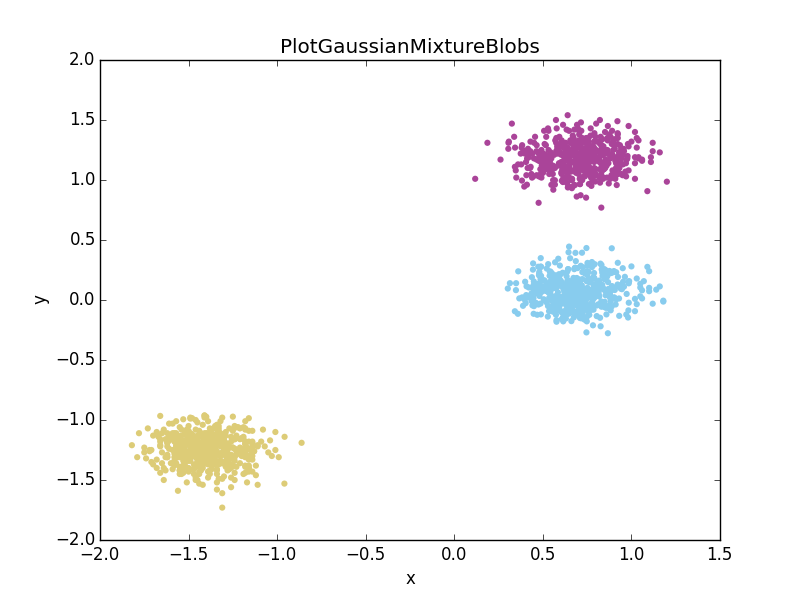
\includegraphics[width=\textwidth]{images/PlotGaussianMixture.png}
\end{frame}

\begin{frame}[fragile]
  \frametitle{Means Shift Clustering Example}
  This is the postprocessor that calculates the Means Shift clustering:
  \lstinputlisting[firstline=15, lastline=22, style=XML]{../../misc/example/cluster/test_dataMiningMeanShift.xml}
\end{frame}

\begin{frame}
  \frametitle{Means Shift Cluster Example Output}
  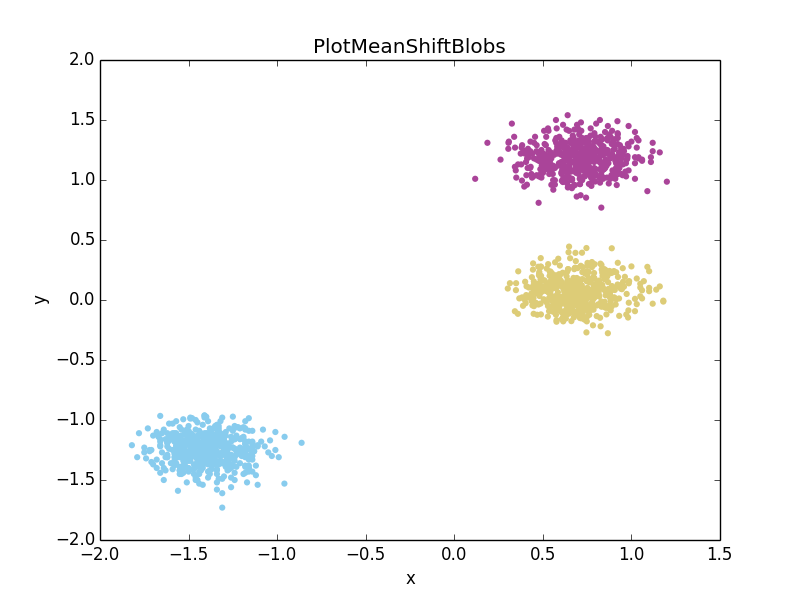
\includegraphics[width=\textwidth]{images/PlotMeanShift.png}
\end{frame}

\begin{frame}[fragile]
  \frametitle{K-Means Clustering Example}
  This is the postprocessor that calculate the K-Means clustering:
  \lstinputlisting[firstline=37, lastline=47, style=XML]{../../misc/example/cluster/test_dataMiningKMeans.xml}
\end{frame}

\begin{frame}
  \frametitle{K-Means Cluster Example Output}
  \includegraphics[width=\textwidth]{images/PlotKMeans.png}
\end{frame}

\section{Dimentionality Reduction Example}

\begin{frame}[fragile]
  \frametitle{Dimentionality Reduction Example}
  This is the postprocessor that decreases the dimentionality:
  \lstinputlisting[firstline=23, lastline=29, style=XML]{../../misc/example/cluster/test_dataMiningExactPCA.xml}
\end{frame}

\begin{frame}
  \frametitle{Exact PCA Dimentionality Reduction Example Output}
  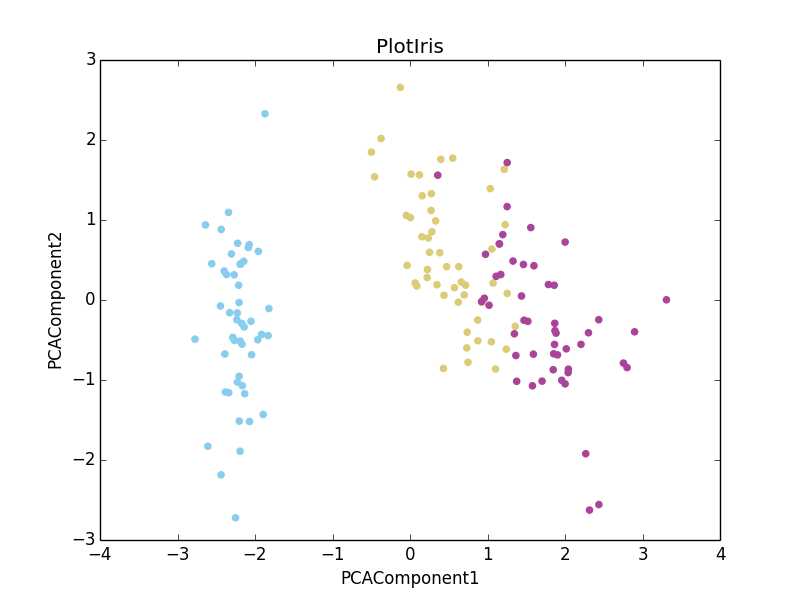
\includegraphics[width=\textwidth]{images/PlotExactPCA.png}
\end{frame}

\section{Basic Statistics with Time Dependence in RAVEN}

\begin{frame}
  \frametitle{Basic Statistics with Time Dependence}
  \begin{itemize}
  \item RAVEN calculates statistics at each time
  \item Allows trends in the data to be seen
  \end{itemize}
\end{frame}

\begin{frame}[fragile]
  \frametitle{Basic Statistics Example}
  This is the postprocessor that calculates the time statistics:
  \lstinputlisting[firstline=13, lastline=19, style=XML]{../../misc/example/temporalBasicStatistics.xml}

\end{frame}

\begin{frame}
  \frametitle{Example Input}
  \begin{itemize}
  \item Contains 100 x,y coordinates
  \item Has timestep data for 100 steps of 0.1
  \end{itemize}
  Play Movie \movie[externalviewer]{(MPEG-1)}{time_data.mpg} \movie[externalviewer]{(Theora)}{time_data.ogg}
\end{frame}

\begin{frame}
  \frametitle{Example Output}
  \begin{columns}
    \column{.5\textwidth}
    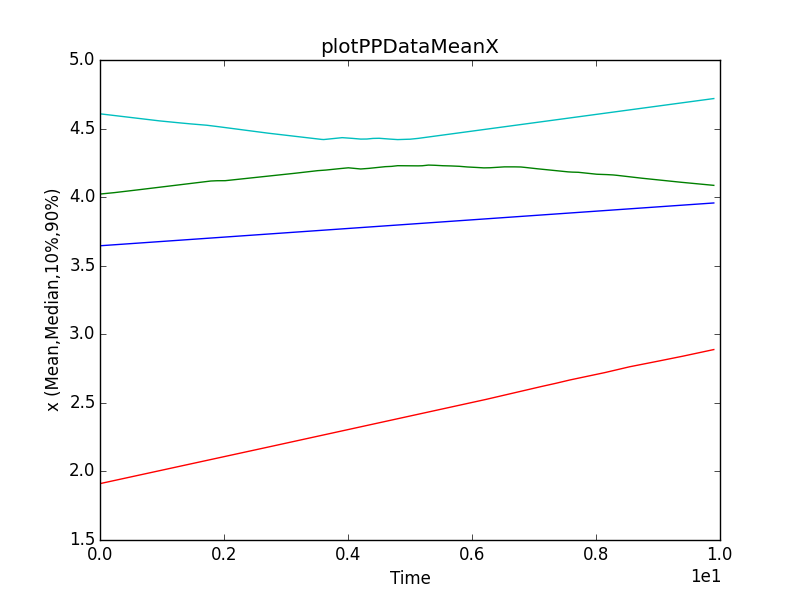
\includegraphics[height=4cm]{images/plotPPDataMeanX.png}
    \column{.5\textwidth}
    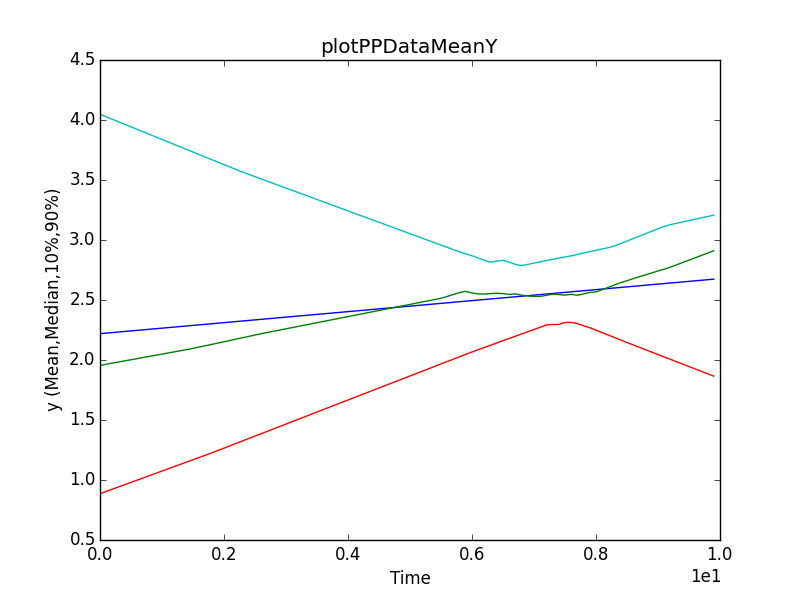
\includegraphics[height=4cm]{images/plotPPDataMeanY.png}
  \end{columns}
\end{frame}
%Basic statistics with time dependence
%%Show example
%%Show input
%%Show output graph

\begin{frame}
  \frametitle{Questions?}
\end{frame}

\end{document}
